% Appendix Template

\chapter{Results of experiment 2.3} % Main appendix title

\label{Appendix2-3} % Change X to a consecutive letter; for referencing this appendix elsewhere, use \ref{AppendixX}

\begin{figure}[th]
\centering
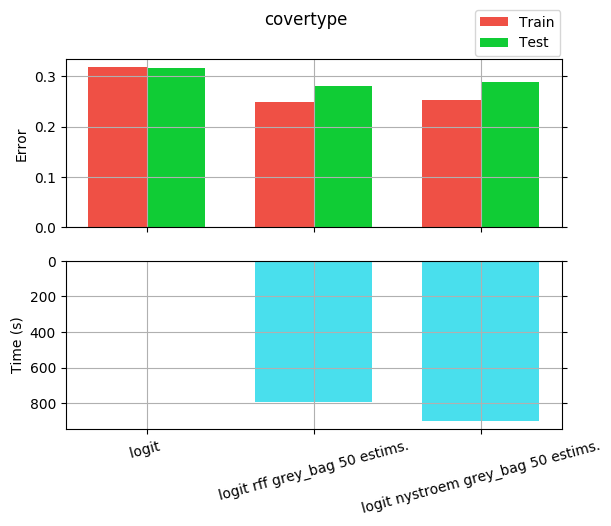
\includegraphics[scale=\imgscale]{Figures/2_3/covertype}
\decoRule
\caption[2.3 covertype]{Logistic Regression with Grey Bag model}
\label{fig:2_3_covertype}
\end{figure}

\begin{figure}[th]
\centering
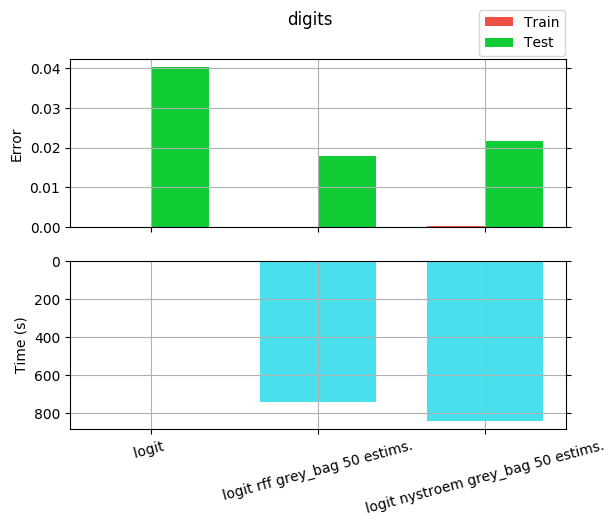
\includegraphics[scale=\imgscale]{Figures/2_3/digits}
\decoRule
\caption[2.3 digits]{Logistic Regression with Grey Bag model}
\label{fig:2_3_digits}
\end{figure}

\begin{figure}[th]
\centering
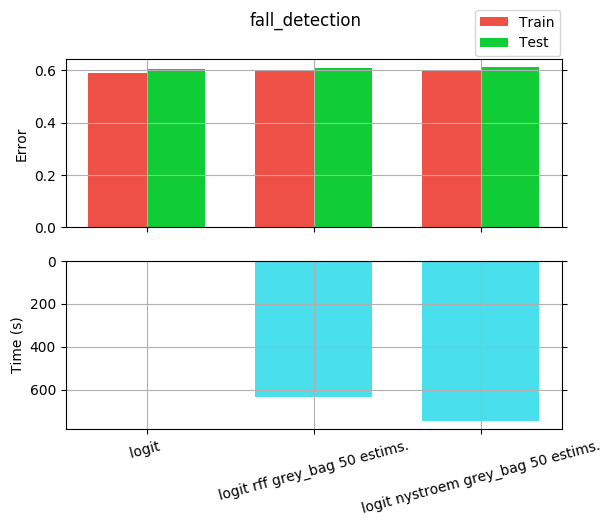
\includegraphics[scale=\imgscale]{Figures/2_3/fall_detection}
\decoRule
\caption[2.3 fall\tu detection]{Logistic Regression with Grey Bag model}
\label{fig:2_3_fall_detection}
\end{figure}

\begin{figure}[th]
\centering
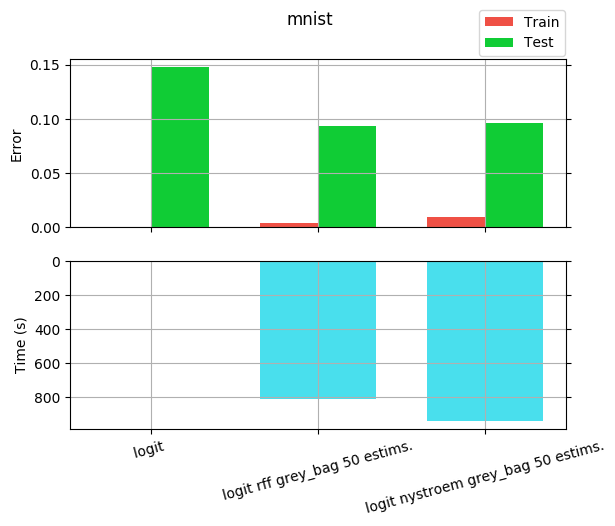
\includegraphics[scale=\imgscale]{Figures/2_3/mnist}
\decoRule
\caption[2.3 mnist]{Logistic Regression with Grey Bag model}
\label{fig:2_3_mnist}
\end{figure}

\begin{figure}[th]
\centering
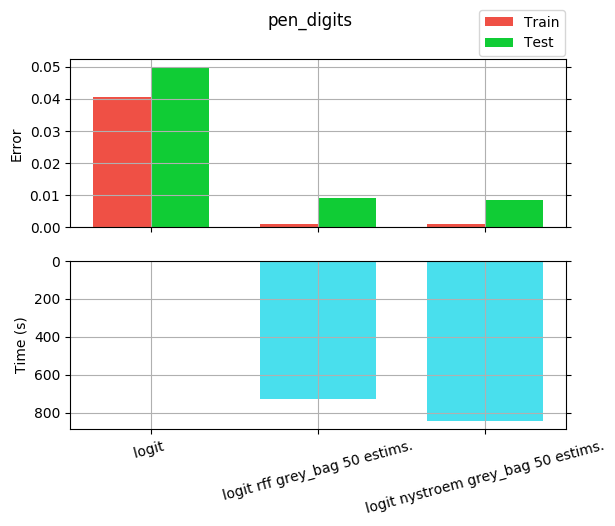
\includegraphics[scale=\imgscale]{Figures/2_3/pen_digits}
\decoRule
\caption[2.3 pen\tu digits]{Logistic Regression with Grey Bag model}
\label{fig:2_3_pen_digits}
\end{figure}

\begin{figure}[th]
\centering
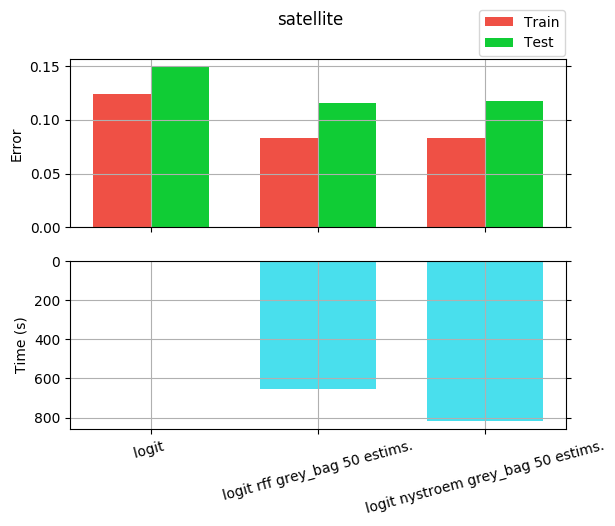
\includegraphics[scale=\imgscale]{Figures/2_3/satellite}
\decoRule
\caption[2.3 satellite]{Logistic Regression with Grey Bag model}
\label{fig:2_3_satellite}
\end{figure}

\begin{figure}[th]
\centering
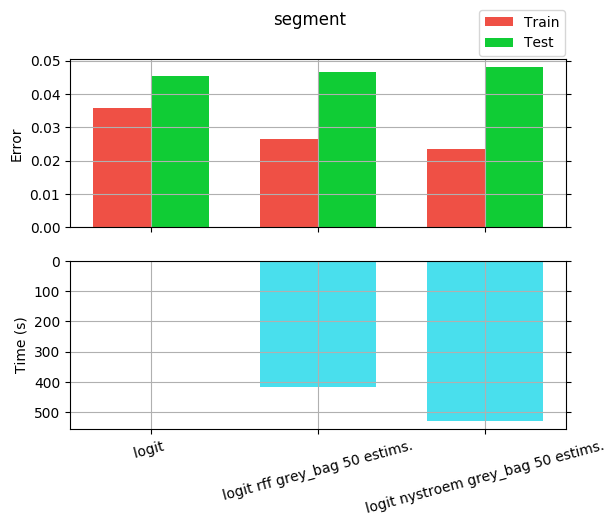
\includegraphics[scale=\imgscale]{Figures/2_3/segment}
\decoRule
\caption[2.3 segment]{Logistic Regression with Grey Bag model}
\label{fig:2_3_segment}
\end{figure}

\begin{figure}[th]
\centering
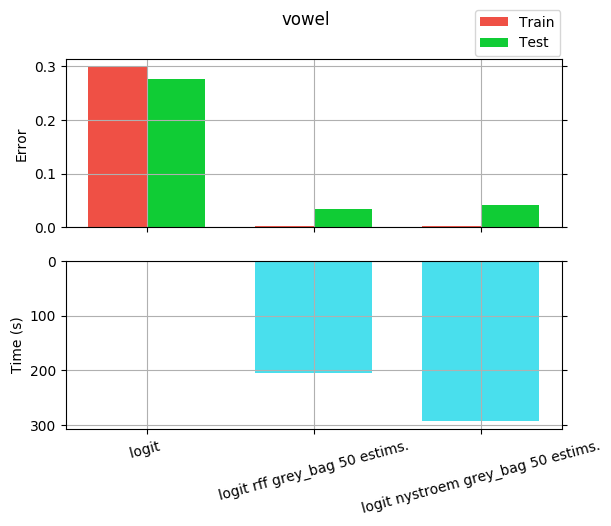
\includegraphics[scale=\imgscale]{Figures/2_3/vowel}
\decoRule
\caption[2.3 vowel]{Logistic Regression with Grey Bag model}
\label{fig:vowel}
\end{figure}
